\documentclass[10pt,a4paper]{scrbook}
\usepackage[utf8]{inputenc}
\usepackage{amsmath,amssymb,amsfonts} % For math
\usepackage{listings} % For code
\usepackage{hyperref} % For links
\usepackage{graphicx} % For images
\usepackage{xcolor}   % For colored text
\usepackage[top=0.5cm]{geometry} % To adjust margins
\geometry{a4paper, left=30mm, right=25mm, top=30mm, bottom=30mm}

% Set up code block styling
\lstset{
    basicstyle=\ttfamily,
    frame=single,
    backgroundcolor=\color{gray!10},
    language=Python,
    breaklines=true
}

% Title page setup
\title{Evolutionary Dynamics of Microbes}
\author{Otto X. Cordero}
\date{\today}

\begin{document}

\frontmatter
% Redefine the clearpage to avoid blank pages
\let\cleardoublepage\clearpage
\maketitle
\tableofcontents

\mainmatter

% Chapter 1: Introduction
\chapter{Introduction}

The goal of this class is to provide students with a conceptual framework and language to think about evolution in a structured and quantitative way. By the end of the class, you should be able to make informed predictions, anticipate and interpret the outcome of experiments, and identify patterns in data related to evolutionary processes.

We will walk through several key concepts in evolutionary theory, understanding their origins and why they remain relevant. We will also explore foundational papers, first focusing on experimental evolution and later shifting to the study of evolution in natural systems using genomic data.

\section{What is Evolution?}
In the literature, evolution is often defined as the “change in allele frequencies” in a population over time. While this definition captures the outcome of evolutionary processes, it doesn’t fully explain the underlying mechanisms.

A broader and more process-based definition is: 

\emph{Evolution is a process that occurs in populations where individuals reproduce, acquire heritable mutations, and die. These processes imply competition for survival and reproduction across generations. Whenever these ingredients are present, evolution can occur—whether in biological entities, words, ideas, or cultures.}

This definition emphasizes that evolution is a general process and can apply beyond biological systems, such as political movements, languages, or market dynamics. A key variable in this definition is the "population". What is a population, in this context? A population, in evolutionary terms, is a group of individuals who compete for survival and reproduction across generations. These individuals share a common environment and resources, creating a system where interactions influence their reproductive success. 

\subsection{The Evolution of Languages: A Model to Ground our Intuition about Evolutionary Dynamics}

The evolution of languages provides a compelling analogy to biological evolution, demonstrating that evolutionary principles extend far beyond the realm of genetics. Languages, like biological organisms, there are populations of symbols and ideas expressed with these symbols that undergo a process of gradual change over time, driven by variation, transmission, and competition. These processes closely mirror the dynamics observed in natural populations, highlighting the generality of evolutionary mechanisms.

\subsubsection{Variation and Mutation in Languages}

Languages evolve through the gradual accumulation of small changes—often referred to as "mutations" in linguistic terms. These changes can occur in pronunciation, grammar, vocabulary, or syntax. For example, a new word might enter a language due to cultural contact or technological innovation, much like a mutation introduces a new allele into a population's gene pool. Over time, linguistic variations accumulate, leading to the emergence of dialects and, eventually, entirely distinct languages.

Just as in biological evolution, not every change is retained in the population. Some linguistic mutations spread and become fixed in a population, while others fade out. The factors that determine whether a change spreads (analogous to natural selection) can include social, cultural, or practical pressures.

\subsubsection{Transmission: Language as Inheritance}

The transmission of language from one generation to the next parallels the inheritance of genetic information. Language is passed down through learning and imitation, much like genetic material is passed from parent to offspring. However, just as genetic transmission is imperfect, language transmission introduces errors or variations, which can accumulate and lead to significant changes over many generations.

This process is not limited to vertical transmission from parent to child; horizontal transmission (similar to horizontal gene transfer in biology) occurs when languages borrow words, structures, or idioms from one another, especially when populations are in contact. For example, the English language has incorporated vocabulary from Latin, French, and many other languages over centuries.

\subsubsection{Selection and Competition in Language Evolution}

Languages, like organisms, compete with one another. In multilingual regions, certain languages may dominate due to political, economic, or social factors, leading to the extinction of other languages. This is analogous to natural selection, where advantageous traits spread through a population while less advantageous traits are lost. In the context of language, selection operates on a variety of factors: ease of communication, adaptability to new contexts, or the influence of powerful cultural or political entities.

For example, Latin evolved into the Romance languages (French, Spanish, Italian, etc.), but the spread of these languages did not occur evenly. Some dialects dominated others, much like how certain species outcompete others for resources.

\subsubsection{Language Divergence and Speciation}

The process of linguistic divergence mirrors the biological concept of speciation. As groups of people become isolated from one another, their languages change independently, eventually becoming mutually unintelligible. This is akin to the genetic divergence that occurs when populations of a species are geographically separated, leading to the formation of new species.

The Romance languages, which evolved from Latin, provide an example of this process. As the Roman Empire declined, isolated populations in Europe began to speak increasingly distinct dialects of Latin. Over time, these dialects became separate languages, like French, Spanish, and Italian, due to both geographic and cultural separation.

\begin{figure}
    \centering
    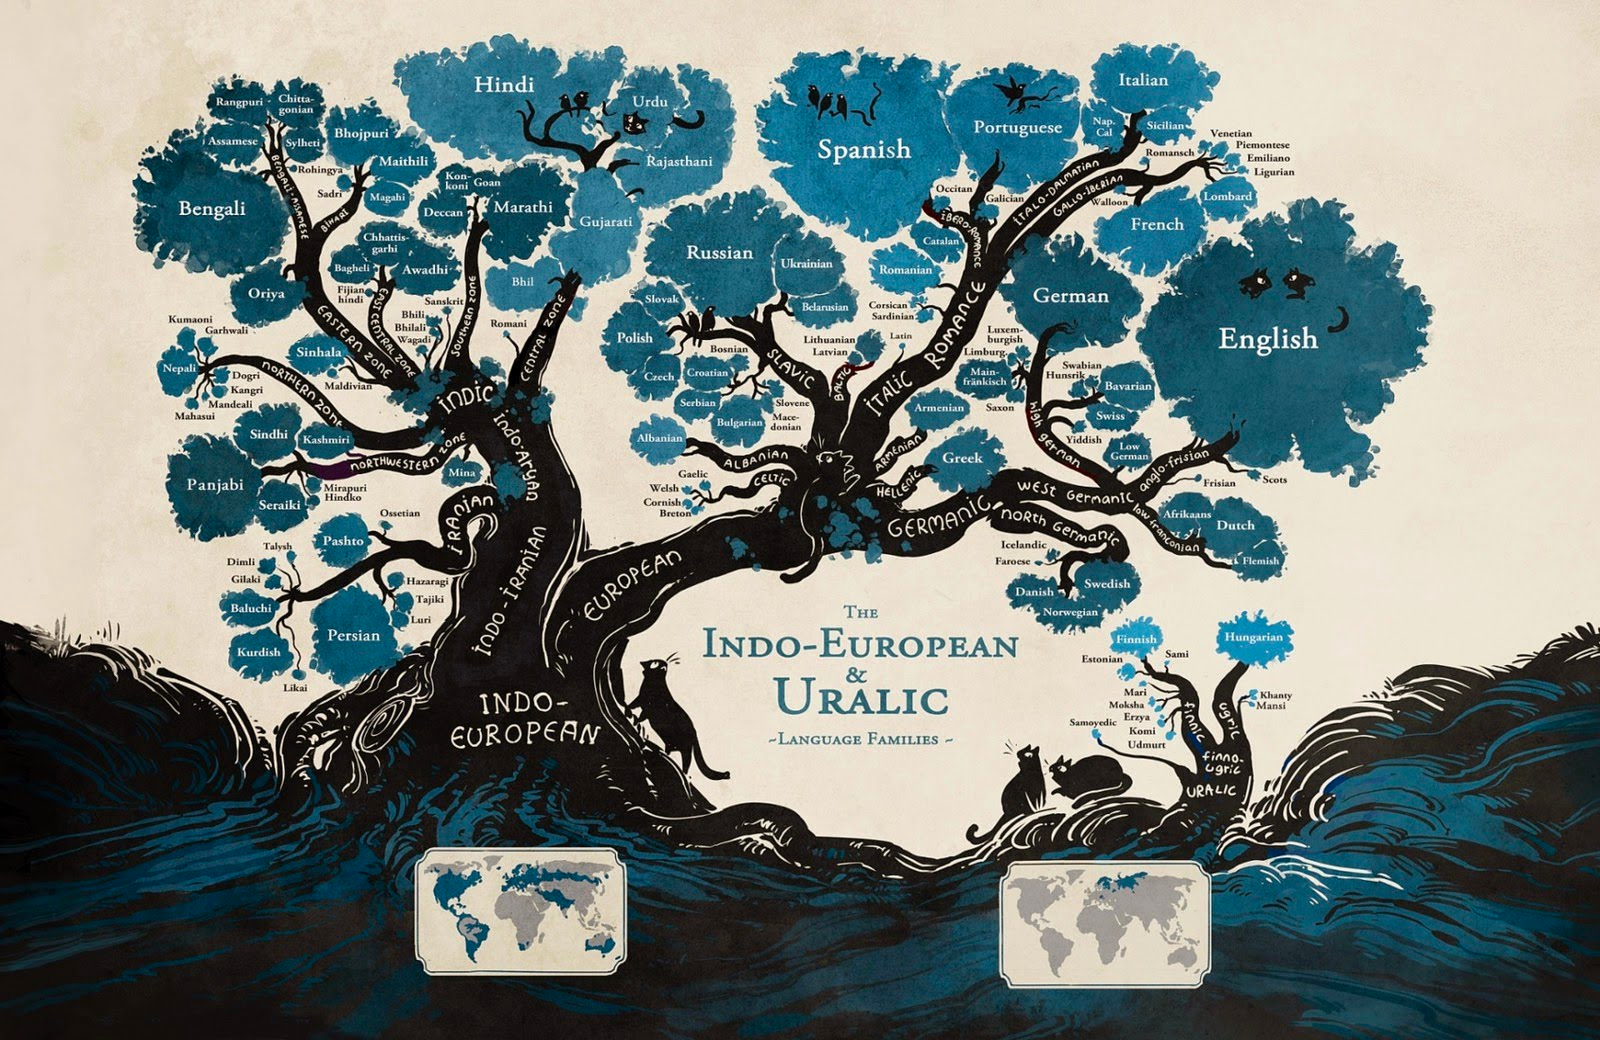
\includegraphics[width=0.75\linewidth]{image.png}
    \caption{Evolution is not limited to biological entities with DNA. No sir! Cultures, and their numerous artifacts (technologies, languages, political ideas, etc.) are subject to the same principles of evolutionary dynamics that operate on living beings. Because we have an easier time thinking intuitively about changes in languages or technology, it is often useful to ground our intuition about evolution in these examples. For instance, think about the evolution of first \href{https://www.pnas.org/doi/abs/10.1073/pnas.1507143112}{name frequencies}}
    \label{fig:LangTree}
\end{figure}

\subsubsection{General Evolutionary Dynamics}

The evolution of languages illustrates that evolutionary dynamics—variation, transmission, selection, and divergence—are not confined to biology. These processes are fundamental to any system where information is passed down through generations, subject to change, and influenced by environmental or social pressures. Whether it's genes, languages, ideas, or cultures, the mechanisms of evolution apply universally.

The study of language evolution thus serves as a powerful analogy for understanding biological evolution and reinforces the idea that evolution is a general process governing many systems beyond life itself (Figure~\ref{fig:LangTree}). Just as species evolve through natural selection and genetic drift, languages evolve through cultural selection and random changes. This highlights the robustness of evolutionary theory as a framework for understanding change across a wide variety of systems.

\begin{figure}
    \centering
    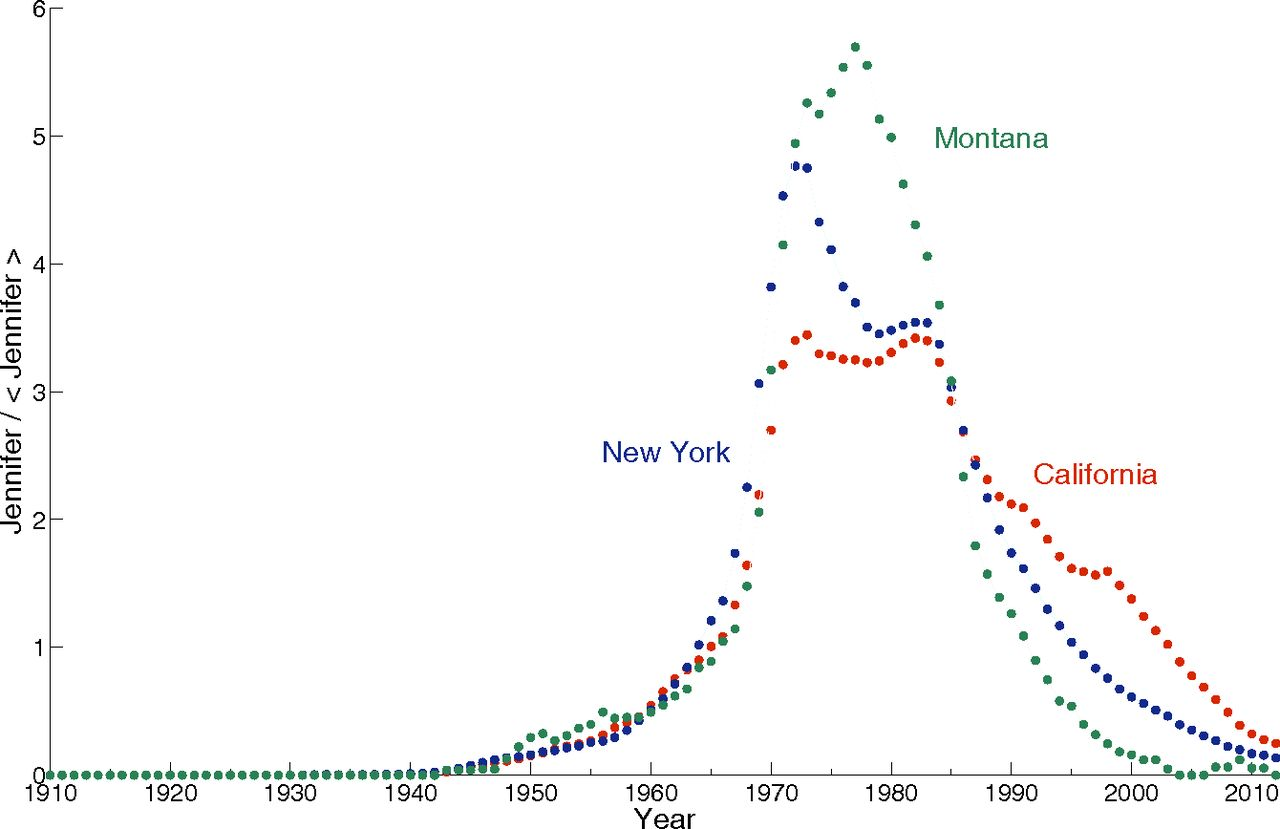
\includegraphics[width=0.75\linewidth]{Parisi.png}
    \caption{Frequency of baby names normalized by their mean (think of it as the reproductive success of the names). Names compete for babies, and the dynamics observed in the figure are the result of an evolutionary process that determines the reproductive success of baby names per generation. What this figure shows is that that reproductive success is variable in time, and most likely a function of the name frequency in the population (a name is not very attractive if everyone has it, plus, people don't want to be named like their grand parents (e.g. how many people named Mildred or Earl do you know?). This is an example of what is called Frequency Dependent Selection, an extremely relevant form of selection for microbes}
    \label{fig:enter-label}
\end{figure}

% Chapter 2: Key Variables and Processes in Evolution
\chapter{Key Variables and Processes in Evolution}

\section{Genetic Drift}

As exemplified for the case of languages, populations can change in their composition through \emph{selection} and pure randomness. We refer to this randomness as \emph{Genetic Drift}. Genetic drift refers to the random fluctuation of allele frequencies in a population from one generation to the next due to chance events. Unlike natural selection, which favors certain genetic variants, genetic drift acts indiscriminately and can cause variants to increase or decrease in frequency purely by random chance. This stochastic process is particularly impactful in small populations, where the random sampling of alleles from one generation to the next can lead to significant changes in allele frequencies over relatively short periods.

Through out this class, we will the Wright-Fisher (WF) model to illustrate basic concepts in evolution, concepts like drift. The reason why we do this is two-fold:  simple models such WF, although highly idealized, allow for a precise definition of the concepts and derivation of the formulas relating processes and variables. The second reason is that the quantitative theory of evolution (for the most part encompassed by "population genetics") is based on such simple models. Thus, using this models for learning can be used to understand where current theory frameworks come from, as well as their power and their limitations as explanations for real-world phenomena.

\subsection{The Wright-Fisher Model for Non-Sexual Populations}

The \textit{Wright-Fisher model} is a foundational model in population genetics that describes how allele frequencies change across generations due to genetic drift in finite populations. When applied to non-sexual (asexual or clonal) populations, the model simplifies to tracking how alleles propagate across generations through clonal reproduction, where each individual passes on its genetic material directly to its offspring.

\subsubsection{Key Assumptions of the Wright-Fisher Model}

\begin{itemize}
    \item \textbf{Finite Population Size}: The population consists of \(N\) individuals, and the model tracks the changes in allele frequencies across generations in this finite population. Each individual in the next generation is an exact clone of an individual from the previous generation.
    
    \item \textbf{Non-overlapping Generations}: Individuals reproduce clonally, pass on their alleles to the next generation, and then die. Each generation is completely replaced by the offspring of the previous generation.
    
    \item \textbf{Random Sampling}: In each generation, the alleles that make up the next generation are sampled randomly from the gene pool of the current generation. This means that the next generation's allele frequencies depend on random sampling from the parent generation.
    
    \item \textbf{Neutral Evolution}: In the basic Wright-Fisher model, there is no selection, mutation, or migration. Allele frequencies change solely due to the randomness of inheritance, i.e., genetic drift.
\end{itemize}

\subsubsection{Mathematical Description}

In a non-sexual population of \(N\) individuals, we track the frequency of a particular allele \(A\). Let \(p_t\) represent the frequency of allele \(A\) in generation \(t\). The frequency of allele \(A\) in the next generation, \(p_{t+1}\), depends on how many copies of \(A\) are sampled to form the next generation. This process is modeled as a binomial random variable, where the number of individuals carrying allele \(A\) in generation \(t+1\) is:

\begin{equation}
X_{t+1} \sim \text{Binomial}(N, p_t)
\end{equation}

where:
\begin{itemize}
    \item \(X_{t+1}\) is the number of individuals with allele \(A\) in generation \(t+1\),
    \item \(N\) is the population size, and
    \item \(p_t\) is the frequency of allele \(A\) in generation \(t\).
\end{itemize}

The frequency of allele \(A\) in the next generation is then:

\begin{equation}
p_{t+1} = \frac{X_{t+1}}{N}
\end{equation}

This binomial sampling process captures the randomness of reproduction, where \(p_{t+1}\) is expected to be close to \(p_t\), but fluctuates due to the inherent randomness of genetic drift.

One of the ways in which we are going to take advantage of the WF models is that it allows for a simple graphical representation of evolution – under the model assumptions of course. Figure~\ref{fig:WF1} shows an example of this diagram. In it, columns correspond to generations and dots to individuals. Lines connect parents with their offsprings, such that you can follow the ancestry back in time and see who are the common ancestors of the current population. When the lines \emph{coalesce} onto one single individual, that individual is said to be the Most Recent Common Ancestor of the extant (i.e. current) population. 

When ancestry lines arrive to a common ancestor we say the lineages coalesce. There is ample body of theory in population genetics about the coalescence process (it's called coalescence theory), that we won't discuss here. However, as you will see below, we will talk about \emph{coalescence times}. This refers to the number of generations back in time needed for the population to coalesce. In the example shown in Figure~\ref{fig:WF1}, coalescence time is 15 generations.

\begin{figure}[htbp]
    \centering
    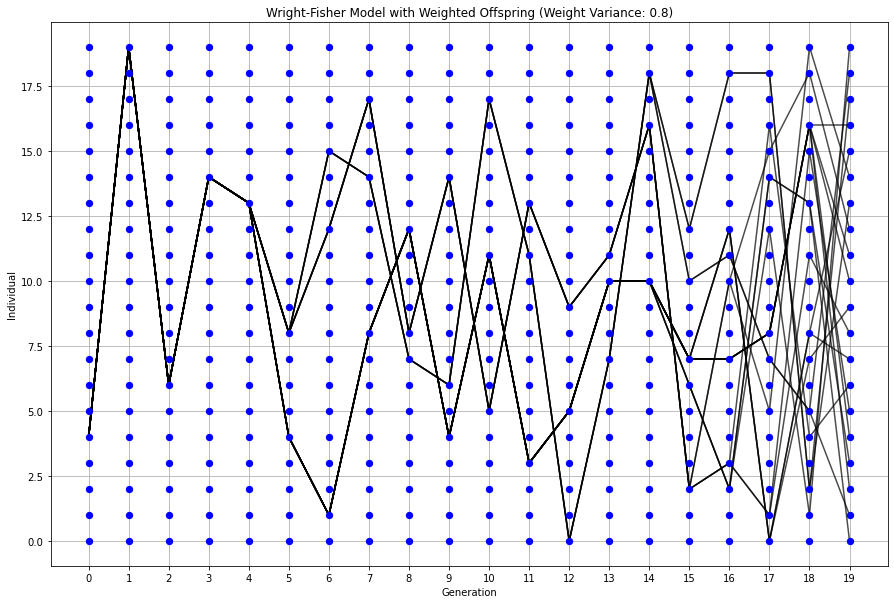
\includegraphics[width=0.8\textwidth]{WF1.png}  % Replace with your image file
    \caption{An graphical representation of a WF process. In this figure, the population of 20 individuals can be traced back to a most recent common ancestor (MRCA) at generation 4, where the lines coalesce to a single parent. As we will see below, the effective population size is a measure of how variance in the sampling process (variability in number of offsprings per individual in a given generation), or related to this, the time to coalesce to a common ancestor. The current simulation is performed with relatively high variance, so that the coalescence time is short enough to occur within the 20 generations of this simulation}
    \label{fig:WF1}
\end{figure}

\subsection{Population Bottlenecks and Effective Population Size}

A \textit{population bottleneck} occurs when a population experiences a sharp reduction in size due to events such as natural disasters, disease outbreaks, or habitat loss. These events drastically affect the \emph{effective population size} (\(N_e\)) in ways that persist even after the population recovers. A bottleneck has several critical effects on \(N_e\), which we will explore in detail.

\begin{figure}
    \centering
    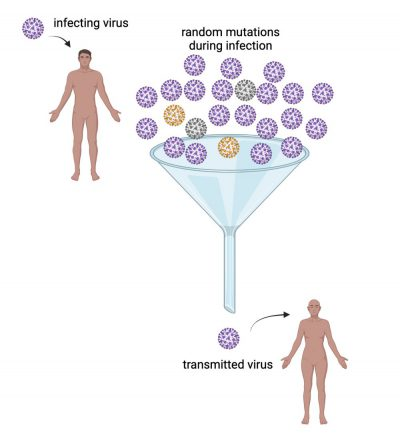
\includegraphics[width=0.5\linewidth]{VirusBottleneck.png}
    \caption{Transmission imposes a significant bottleneck for pathogens like viruses, where typically one or a few individuals found a population inside a host. This population goes many rounds of mutation and diversification before spreading, again, through sharp bottlenecks. Same is true for many pathogens. Figure by \href{https://inside.upmc.com/massive-numbers-of-new-covid-19-infections-not-vaccines-are-the-main-driver-of-new-coronavirus-variants/}{Vaughn Cooper}}
    \label{fig:bottleneck1}
\end{figure}

\subsubsection{Immediate Reduction in \(N_e\)}

During a bottleneck, the number of individuals that survive and reproduce is drastically reduced. Since \(N_e\) reflects the number of individuals effectively contributing to the next generation, a bottleneck results in a temporary but significant reduction in \(N_e\). This immediate drop in \(N_e\) increases the rate of genetic drift, causing random changes in allele frequencies and reducing genetic diversity.

\subsubsection{Loss of Genetic Diversity}

A population bottleneck reduces genetic diversity because only a small subset of the original population contributes alleles to the next generation. Some alleles (especially rare ones) may be lost entirely, while others may become fixed purely by chance. This loss of genetic diversity persists even after the population size recovers, meaning the genetic diversity post-bottleneck is often much lower than before the event. See the section on loss of Heterozygosity for a more precise discussion about the relationship between \(N_e\) and the loss of genetic diversity. 

\subsubsection{Long-Term Effects on \(N_e\)}

Even if the population size \(N\) recovers quickly after the bottleneck, the effective population size \(N_e\) remains reduced for several generations. This is because \(N_e\) is not just determined by the current population size but also by the genetic diversity that was lost during the bottleneck. It takes many generations of random mating and genetic recombination for \(N_e\) to approach the new census population size.

In fact, \(N_e\) over time is influenced by historical fluctuations in population size. When calculating the long-term effective population size (\(N_{e,\text{long-term}}\)) for a population that has gone through bottlenecks, the harmonic mean of population sizes across generations is used:

\begin{equation}
N_{e,\text{long-term}} = \frac{T}{\frac{1}{N_{e1}} + \frac{1}{N_{e2}} + \dots + \frac{1}{N_{et}}}
\end{equation}

where \(T\) is the total number of generations, and \(N_{e1}, N_{e2}, \dots, N_{et}\) are the effective population sizes in each generation. The harmonic mean ensures that periods of low population size (like bottlenecks) have a disproportionate impact on the overall \(N_e\).

Thus, even if the population size increases after a bottleneck, the overall \(N_e\) will be skewed by the very small population sizes during the bottleneck. It takes time for \(N_e\) to recover, and the reduction in genetic diversity may be permanent.

\subsubsection{First-Principle Derivation of the Harmonic Mean}

The harmonic mean arises from the fact that \textit{genetic drift}—the random fluctuation in allele frequencies from one generation to the next—has a disproportionately strong effect during periods when the population size is small. To understand this, let’s explore how drift works in principle.

\paragraph{Genetic Drift and Population Size:}
Genetic drift causes alleles to randomly fluctuate in frequency from generation to generation, and the strength of drift is inversely related to population size. In smaller populations, random sampling errors in reproduction have a larger impact on allele frequencies, leading to faster changes.

\paragraph{Effect of Population Size Over Multiple Generations:}
When populations fluctuate in size over time, smaller population sizes contribute more significantly to overall genetic drift. Therefore, when calculating \(N_e\), we must account for the periods of small population size more heavily. This is done by using the harmonic mean of the population sizes over time, which gives greater weight to smaller sizes.

Thus, the harmonic mean \(N_e\) is given by:

\begin{equation}
N_e = \frac{T}{\sum_{i=1}^{T} \frac{1}{N_i}}
\end{equation}

where \(N_i\) is the population size in generation \(i\). The harmonic mean reflects the fact that smaller population sizes, where genetic drift is stronger, have a disproportionate effect on the overall genetic drift over time.

\subsubsection{Consequences of Bottleneck in Microbes}

Consider a bacterial population that experiences a bottleneck when only a few cells survive after exposure to an antibiotic. Even if the population quickly recovers in numbers, the small number of surviving cells that contribute to the next generation means that:

\begin{itemize}
    \item The \textit{effective population size} \(N_e\) is drastically reduced, even though the total number of cells may quickly return to its original size.
    \item The \textit{genetic diversity} of the population is significantly lower because only the alleles carried by the few surviving cells will be passed on to future generations. Many other alleles are lost.
    \item Over time, even as the population grows back to its original size, the effect of the bottleneck on \(N_e\) persists, leading to stronger genetic drift and reducing the population's ability to adapt to new challenges.
\end{itemize}

\subsubsection{Drift and the Loss of Diversity}

Genetic diversity, or Heterozygosity, \(H\), can be quantified as the probability that two randomly chosen alleles from the population are different. To be clear, this means the following: sample two individuals (with replacement) at random from the population, observe their allele variants and a given locus. For a population with two alleles \(A_1\) and \(A_2\), with frequencies \(p\) and \(q = 1 - p\), respectively, heterozygosity is given by:

\begin{equation}
H = 2pq = 2p(1 - p)
\end{equation}

This is because you can sample allele \(A_1\) with probability \(p\), and subsequently \(A_2\) with probability \(1-p\), or you can also sample the reverse, first \(A_2\) and then \(A_1\), which is why there is a 2 in front of the formula. 

In a clonal population, genetic drift causes heterozygosity to decrease over time, as allele frequencies fluctuate due to random sampling. More precisely, the expected heterozygosity in the next generation, \(H_{t+1}\), is:

\begin{equation}
H_{t+1} = H_t \left( 1 - \frac{1}{N_e} \right)
\end{equation}

Iterating this equation over \(t\) generations gives:

\begin{equation}
H_t = H_0 \left( 1 - \frac{1}{N_e} \right)^t
\end{equation}

For large \(N_e\), we approximate using the exponential function:

\begin{equation}
H_t \approx H_0 e^{-\frac{t}{N_e}}
\end{equation}

Thus, heterozygosity decays exponentially at a rate proportional to \(1/N_e\), meaning that smaller populations experience faster loss of genetic diversity.

\subsubsection{Conclusion}

Population bottlenecks have a profound impact on the effective population size \(N_e\). Even a brief reduction in population size can cause a significant and lasting decrease in \(N_e\), which accelerates genetic drift, reduces genetic diversity, and limits adaptive potential. This effect can persist even after the population size recovers, emphasizing the importance of maintaining large, stable populations to preserve genetic diversity over time.


\subsection{Variance in Reproductive Success and Effective Population Size in Microbes}

Above we saw that $N_e < N$ can be caused by bottlenecks. This is intuitive: for the transmission of information from generation to generation is doesn't matter how large the census population is, what matters is how many parents contribute to the next generation. If only one does, well, all individuals would be descendents from a single clones and $N_e$ = 1. Here, we will see that a high variance in offspring number is equivalent to bottlenecks, in the sense that it can cause some parents to contribute disproportional to the next generation, leading to an increase in drift.  

In a non-sexual population, the relationship between the \emph{effective population size} (\(N_e\)) and the variance in offspring number is can be defined as:
\begin{equation}
\label{Eq1}
N_e = \frac{N}{1 + \frac{\sigma^2}{\mu^2}}
\end{equation}
where:
\begin{itemize}
    \item \(N\) is the census population size,
    \item \(N_e\) is the effective population size,
    \item \(\sigma^2\) is the variance in the number of offspring per individual, and
    \item \(\mu\) is the mean number of offspring per individual (usually \(\mu = 1\) in non-sexual populations).
\end{itemize}

This formula shows that as the variance in offspring number increases, the effective population size \(N_e\) decreases, leading to stronger genetic drift. Conversely, if all individuals contribute approximately the same number of offspring, \(N_e\) will approach \(N\), and the effects of genetic drift will be weaker.

In microbial populations, particularly those that reproduce clonally (such as bacteria), the variance in reproductive success can be high. For example, in an environment like the human gut or a nutrient-rich patch in the soil, only a small subset of bacteria may be actively reproducing, while the rest of the population remains dormant or reproduces at a much lower rate. At the same time, the census population sizes (\textit{N}) can be quite large. For example, \href{https://en.wikipedia.org/wiki/Candidatus_Pelagibacter_communis}{SAR11}, a small $\alpha$-proteobacterium that is abundant in the oceans has \textit{N} of $\sim10^8$  cells of  per liter. In the human gut, cell densities can be $10^{10} - 10^{11}$ cells per gram of intestinal content. Assuming a population contributes even $\sim$0.1\% of the total cell density, we are talking about $10^{7}-10^{8}$ cells per gram. These are extremely high numbers for evolution. Looking back at Eq~\ref{Eq1}, even if the variance in reproductive success per individual (\(\sigma^2\)) was 100 times larger than the mean (\(\mu\)), this would still be an $N_e$ of $10^5-10^6$. Is that high? is that low? Well, the answer depends on how strong selection is, and we should be able to answer this question more precisely when we talk about it later in this chapter, but in the absence of selection, it means  it could still take millions of generations for diversity to drop by, say, 10\% (\(H_t/H_0 = 0.1\)). 

\begin{figure}[htbp]
    \centering
    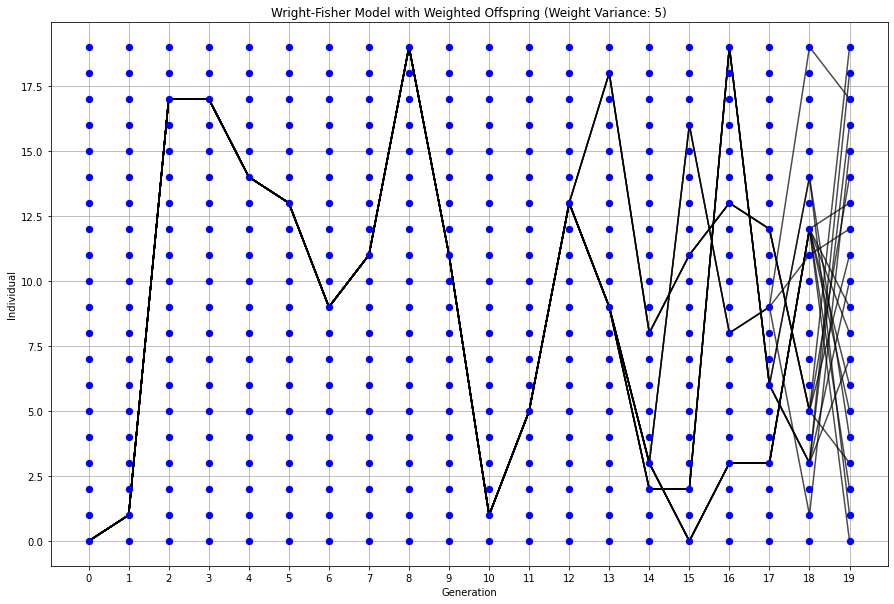
\includegraphics[width=0.8\textwidth]{WF2.png}  % Replace with your image file
    \caption{An graphical representation of a WF process. In this figure, the population of 20 individuals can be traced back to a most recent common ancestor (MRCA) at generation 12, where the lines coalesce to a single parent. This coalescence time is shorter than in Fig~\ref{fig:WF1} because of the high variance in reproductive success (\(\sigma^2\) = 5)}
    \label{fig:WF1}
\end{figure}

\begin{figure}[htbp]
    \centering
    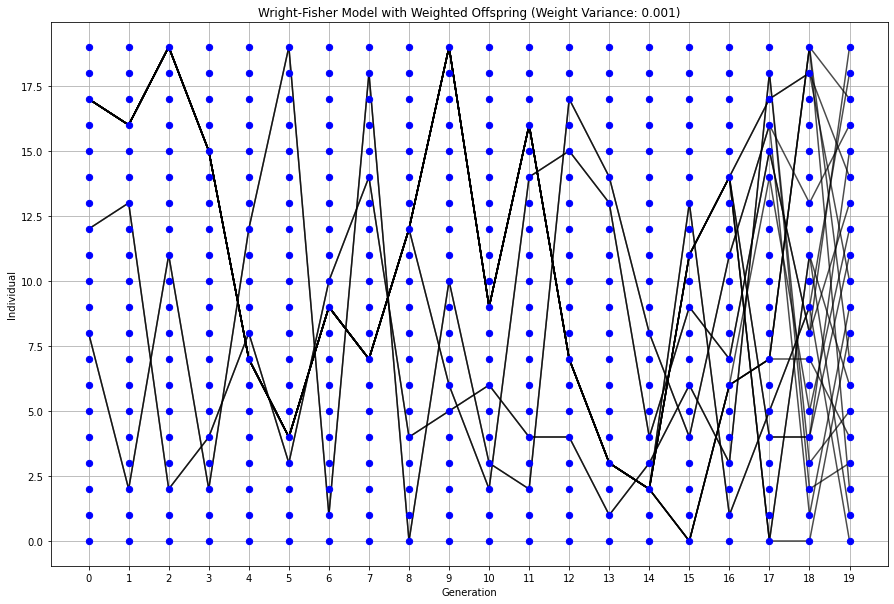
\includegraphics[width=0.8\textwidth]{WF3.png}  % Replace with your image file
    \caption{An graphical representation of a WF process. In this figure, the population does not coalesce in the 20 generations of the simulation. The reason is that the variance in reproductive success is low (\(\sigma^2\) = $10^{-3}$), which implies $N_e$ is large, which implies diversity is preserved for a long time, i.e. coalescence times are long}
    \label{fig:WF1}
\end{figure}

\subsubsection{Impact of \(N_e\) in Non-Sexual Populations}

In non-sexual populations, \(N_e\) plays a key role in shaping evolutionary outcomes:

\begin{itemize}
    \item \textbf{Stronger Drift:} A smaller effective population size means that random changes in allele frequencies (genetic drift) have a stronger effect. This can lead to the rapid loss of genetic diversity and the fixation of neutral mutations.
    
    \item \textbf{Slower Adaptation:} A small \(N_e\) also limits the power of natural selection. In populations where \(N_e\) is small due to high variance in reproductive success, even beneficial mutations may not spread efficiently, as they can be overwhelmed by drift. We will talk more about this when we discuss selection
    
    \item \textbf{Bottlenecks:} In clonal populations, periods of reduced population size (bottlenecks) further reduce \(N_e\), exacerbating the effects of drift. For example, during a population bottleneck, only a few individuals may survive to reproduce, and their offspring will dominate the next generation, dramatically reducing genetic diversity.
\end{itemize}

\subsubsection{Conclusion}

Variance in offspring number is a key determinant of the effective population size (\(N_e\)) in non-sexual populations. As the variance increases, \(N_e\) decreases, and genetic drift becomes a dominant force, leading to the rapid loss of genetic diversity. Understanding the relationship between variance and \(N_e\) is crucial for studying evolutionary dynamics in clonal populations, especially in systems like microbial evolution, where high variance in reproductive success is common.


\subsection{Mutations and Population Diversity}

Mutations introduce new genetic diversity into a population. To be precise in our thinking about this process, let's go back to our Wright-Fisher model. Mutations are introduced with rate \( \mu \) every time an ancestor produces an offspring. Here, \( \mu \) is the rate at which offspring differentiate from their parents. If the organisms had DNA, those differences would be manifested in their genomes, and mutations would lead to an increase in the branch-lengths of the family tree (i.e. the phylogeny). What the basic theory that we can derive with the WF model tells us is that those branch lengths should proportional to the product of the mutation rate \( \mu \) and the effective population size \(N_e\):

\[
\text{Diversity} \propto N_e \times \mu
\]

This is intuitive. The higher the $N_e$ is, the longer the \emph{coalescence times} are, and therefore the longer the history throughout which mutations could have accumulated and contributed to the diversity observed in the current generation. Put differently, if $N_e$ is very small, all members of the current population are descencents of the same few ancestors, and therefore likely to be nearly identical (except for the few mutations that could be introduced in the short coalescence time).

\subsubsection{Can we measure $N_e$?}
The corollary of these ideas is that the standing diversity of a population is not just a function of the rate of diversification, but of its demographic history, and therefore whenever we measure diversity (which as we will see it's easily done from sequence alignments and phylogenies), we are measuring a combination of the intrinsic mutation rate and the effective population size, which captures demographic fluctuations. Thus, we cannot measure \( \mu \) or \( N_e \) from diversity data, only their product. In order to infer \( N_e \), we need a separate, independent measure of \( \mu \). While mutation rates are relatively well-constrained for some organisms in the \href{https://pmc.ncbi.nlm.nih.gov/articles/PMC2932672/}{laboratory}, they can indeed be \href{https://journals.plos.org/plosbiology/article?id=10.1371/journal.pbio.3000617}{variable} and \href{https://onlinelibrary.wiley.com/doi/10.1111/j.1365-2958.2006.05150.x}{evolvable} in nature which complicates estimating $N_e$ from data. But perhaps more importantly, as we will see later, microbial populations can be highly recombinant, which effectively means that different loci can have different lineage histories and coalescence times, i.e. different $N_e$. For these reasons it is actually extremely difficult to measure $N_e$. Philosophically, this poses an interesting question: is there value is having a theory that deals with variables we cannot measure?

\section{Selection}

\end{document}
